\chapter{Implementacija i korisničko sučelje}
		
		
		\section{Korištene tehnologije i alati}
		
			Dio  zadužen za frontend i komunikaciju s korisnikom je ostvaren pomoću knjižnice \href{https://react.dev/}{React}, te je pisan u programskom jeziku
			\href{https:www.typescriptlang.org/}{TypeScript}. React, kao bibilioteka je široko raspostranjen u području stvaranja korisničkog sučelja. Jedna od glavnih prednosti jest objedinjavanje visokih performansi brzine aplikacije, korištenjem 
virtualnog DOM-a, te omogućuje podršku za ponovnu uporabivost komponenti i nadogradnju sustava (zbog svoje enkapsuliranosti). Razvila ga je grupa Meta (Facebook) i naglask se stavlja na njegovu pripadnost knjižnicama, a ne radnim okvirima. \\
			Razvojno okruženje u kojem je pisan cijeli frotend je \href{https://code.visualstudio.com/}{Visual Studio Code}(tzv. VSC). VSC je integrirano razvojno okuženje u vlasništvu tvrtke Microsoft. Danas je to jedna od najkorišenijih tehnologija za uređivanje i pisanje koda, a to je s dobrim razlogom jer on nudi mnoštva ekstenzija za razne programske jezike (pa tako i za TypeScript u kojem je naša aplikacija pisana), ali i jednostavne funkcionalnosti koje ispadaju uvelike korisne te olakšavaju posao pisanja koda, a neke od tih su: debugger, IntelliSense koji služi kao autofill i ugrađena podrška za Git. \\
			Backend sustava pisan je u programskom jeziku \href{https://www.java.com/en/}{Java} korištenjem radnog okvira \href{https://spring.io/projects/spring-boot/}{Spring Boot}. Spring Boot je implementiran kao specijalizacija generaliziranijeg radnog okvira Spring, a omogućuje izradu stand-alone aplikacija. Dobrim dijelom olakšava posao izgradnje sustava jer sam konfigurira funckionalnosti Springa, ali i sam ima već podešene one dijelove web aplikacije koji se učestalo koriste (npr. servleti).\\
			Cijeli backend je pisan u razvojnom okruženju \href{https://www.jetbrains.com/idea/}{InntelliJ IDEA}. To je integrirano razvojno sučelje u vlasništvu kompanije JetBrains, a prevladavajuće je u području pisanja porgrama u Javi i Kotlinu. Velike funkcionalnosti koje koristi su coding assistance, remote cooperation kao i jednostavnost uporabe. \\
			Za dokumentaciju se koristio programski jezik \href{https://www.latex-project.org//}{$LaTeX$}. $LaTeX$ je jezik za pisanje strukturiranih tesktova, piše se kao običan tekst sa dodanom semantičkom strukturom (ne prikazuje se kao konačan proizvod kao npr. Microsoft Word) što mu omogućuje stabilniji rad, a sve što zahtjeva je instalriana distribucija TeX-a; što je u našem slučaju \href{https://miktex.org/}{MiKTeX}. Dokumentacija je pisana u uređivaču teksta zvanom \href{https://www.xm1math.net/texmaker/}{Texmaker} koji se ističe po jednostavnosti pisanju $LaTeX$ dokumenata kao i u svojoj dostupnosti.\\
			Realizacija baze podataka izvedena je U \href{https://www.postgresql.org/}{PostgreSQL-u}. PostgreSQL je open-source sustav za upravljanje relacijama bazama podataka. Uvelike naglasak stavlja na ispunjavanju ACID svojstava pri izvođenju transakcija i pristupačan je za korištenje. Unutar PostgreSQL-a korišten je \href{https://www.pgadmin.org/}{pgAdmin} kao grafički alat za upravljanje bazama podataka i njihovh shema.
			U izradi UML dijagrama korištene su dvije tehnologije: \href{https://astah.net/}{Astah} i \href{https://www.visual-paradigm.com/}{Visual Paradigm}. Oba se alata ističu po svojoj rasprostranjenosti tako što omogućavaju izbor kreiranja svakojakih dijagrama, ali i po svojoj jednostavnosti. Razlika je u tome što je Astah porgram koje se pokreće lokalno na računalu, a Visual Paradigm se pokreće online i sprema trenutne izmjene po izboru lokalno ili na Cloud.\\
			Kako bi se lakše upravljalo verzijama projekta, korišten je \href{https://git-scm.com/}{Git}. Git je besplatan, open source sustav koji se koristi za upravljanje kako manjih, tako i većih projekata. Prednosti su mu brzina, jednostavnost i lakoća upravljanja projektima u timskom radu. Vanjski repozitorij projekta se nalazi na besplatnoj web platformi \href{https://github.com/}{GitHub} koja omogućuje lako upravljanje projektom svim sudionicima repozitorija. \\
			Za produkciju aplikacije korišen je cloud sustav \href{https://render.com/}{Render}. Render olakšava puštanje aplikacija u pogon kako bi bile javno dostupne za pronalazak an internetu. \\
			Kako bi se u timu maksimalno olakšala komunikacija članova kroišen je \href{https://discord.com/}{Discord}. Discord je društvena platforma u kojoj je naglasak na jednostavnosti postizanja glasovne, video i tekstne komunikacije u zajednicama koje se nazivaju serveri kojima se pristupa pomoću poveznice, a omogućuju kavlitetan integritet tima (zajednice).
			\eject 
		
	
		\section{Ispitivanje programskog rješenja}
	
			
			\subsection{Ispitivanje komponenti}
			\textit{Potrebno je provesti ispitivanje jedinica (engl. unit testing) nad razredima koji implementiraju temeljne funkcionalnosti. Razraditi \textbf{minimalno 6 ispitnih slučajeva} u kojima će se ispitati redovni slučajevi, rubni uvjeti te izazivanje pogreške (engl. exception throwing). Poželjno je stvoriti i ispitni slučaj koji koristi funkcionalnosti koje nisu implementirane. Potrebno je priložiti izvorni kôd svih ispitnih slučajeva te prikaz rezultata izvođenja ispita u razvojnom okruženju (prolaz/pad ispita). }
			
			U ovom potpoglavlju razrađeno je testiranje backend dijela aplikacije sa konkretno implementiranim testovima. Testovi su JUnit testovi, a na slici 5.1 prikazan je vremenski interval svakog od 7 testova, kao i verifikacija za njihov prolaz.\\
			\\
			\textbf{Test 1: Metoda koja vraća registrirani gradski ured u bazi podataka}\\
			\\ U ovom je testu cilj bio iz baze podataka "izvući" jedan gradski ured koji odgovara određenim atributima. Dobivena relacije je perotvorena u DTO oblik za lakše rukovanje u sustavu.\\
			\begin{figure}[H]
			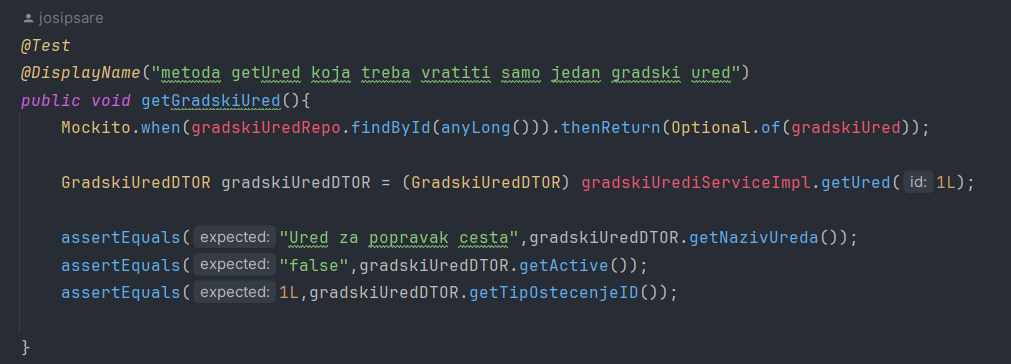
\includegraphics[scale=0.4]{slike/getUred.PNG} %veličina slike u odnosu na originalnu datoteku i pozicija slike
			\centering
			\caption{Pregled gradskog ureda određenih atributa metodom getGradskiUred()}
			\label{fig:implementacija}
		\end{figure}
			
			
			 \textbf{Test 2: Metoda koja provjerava postojanost novostvorenog ureda}\\
			\\ U ovom je testu cilj bio pregledati sadržaj baze podataka nakon stvaranja novog gradskog ureda, kokretnije ispravnost zapisa njegovih atributa.
			
			\begin{figure}[H]
			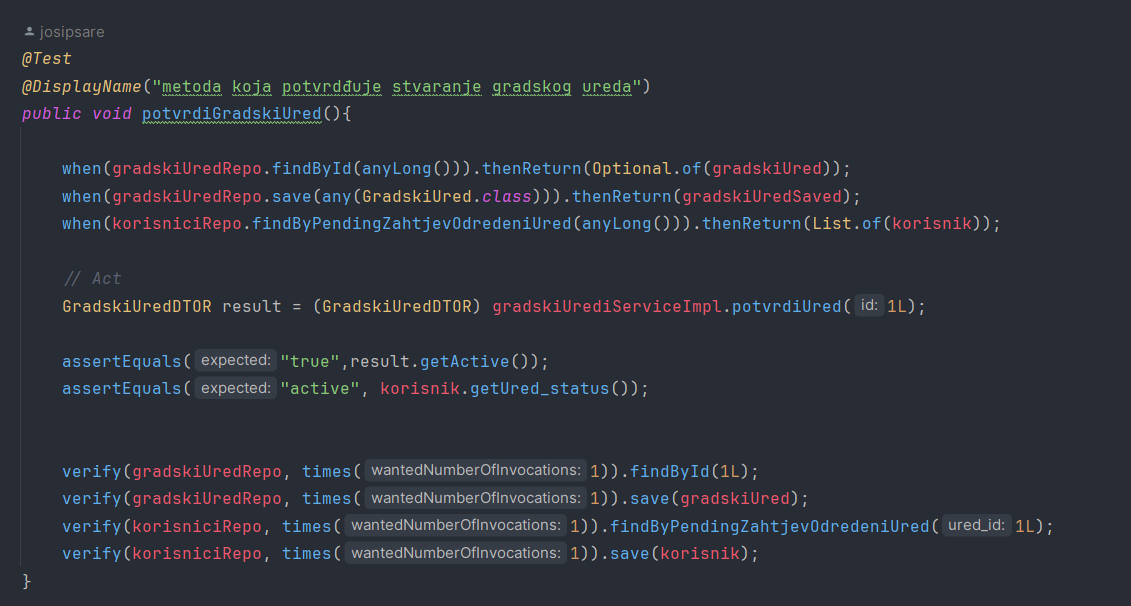
\includegraphics[scale=0.4]{slike/potvrdiUred.PNG} %veličina slike u odnosu na originalnu datoteku i pozicija slike
			\centering
			\caption{Potvrđivanje novonastalog gradskog ureda metodom potvrdiGradskiUred()}
			\label{fig:implementacija}
		\end{figure}
		
		
		\textbf{Test 3: Pretraživanje nepostojećeg korisnika u bazi podataka}\\
			\\ U ovom je testu cilj bio pronaći nepostojećeg korisnika u bazi podataka i uočiti baca li se adekvatna iznimka.
			
			\begin{figure}[H]
			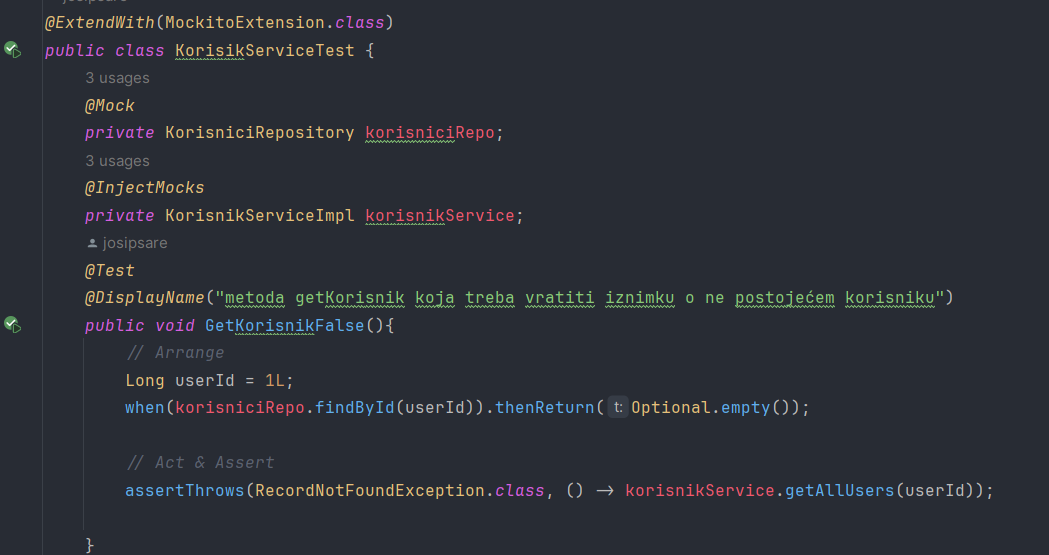
\includegraphics[scale=0.6]{slike/nepostojeciUser.PNG} %veličina slike u odnosu na originalnu datoteku i pozicija slike
			\centering
			\caption{Pregled postojanosti nepostojećeg korisnika}
			\label{fig:implementacija}
		\end{figure}
		
		\pagebreak 
		
		\textbf{Test 4: Pregled svih postojećih korisnika u sustavu}\\
			\\ U testu prikazanom na idućoj slici kreirano više korisnika sa vlastitim atributima. Novonastali korisnici su dodani u listu te je na testa kraju vraćena odgovarajuća lista u koju su dodani spomenuti korisnici kako bi se provejrio zapis objekata u bazi podataka.
			
			\begin{figure}[H]
			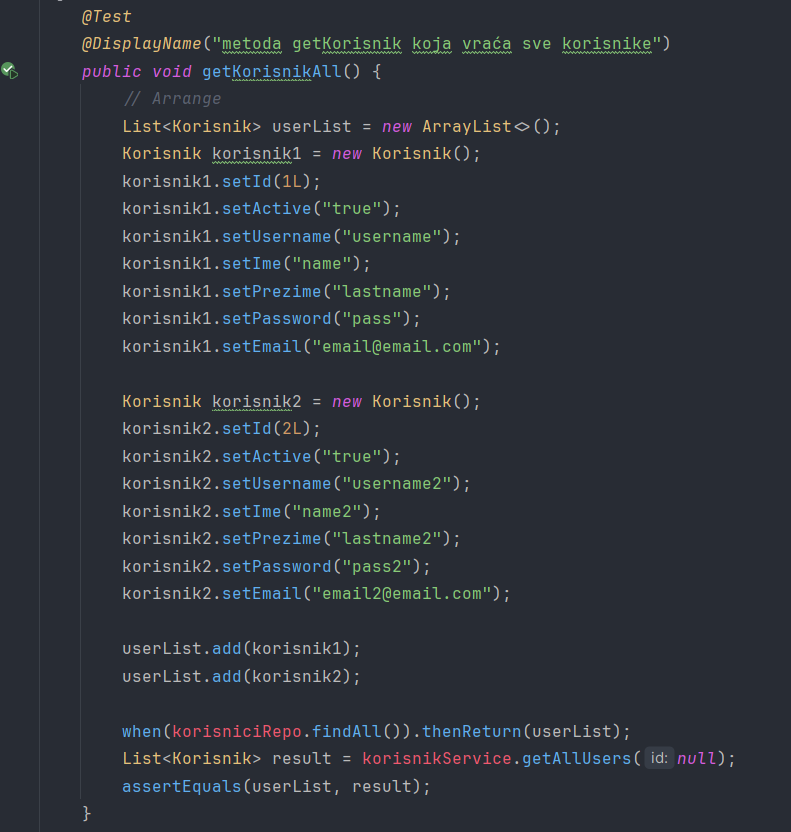
\includegraphics[scale=0.6]{slike/allUsers.PNG} %veličina slike u odnosu na originalnu datoteku i pozicija slike
			\centering
			\caption{Pregled liste svih postojećih korisnika sa svojim atrubutima u sustavu metodom getKorisnikAll()}
			\label{fig:implementacija}
		\end{figure}
		
		\textbf{Test 5: Registracija novog korinsika u sustav}\\
			\\ U testu broj pet kreiran je jedan user sa svojim pripadajućim atributima i spremljen u bazu podataka. Cilj je dobiti istog tog korisnika pretragom po određenom atributu i učiti ispravnost zapisa novonastalog objekta
			
			\begin{figure}[H]
			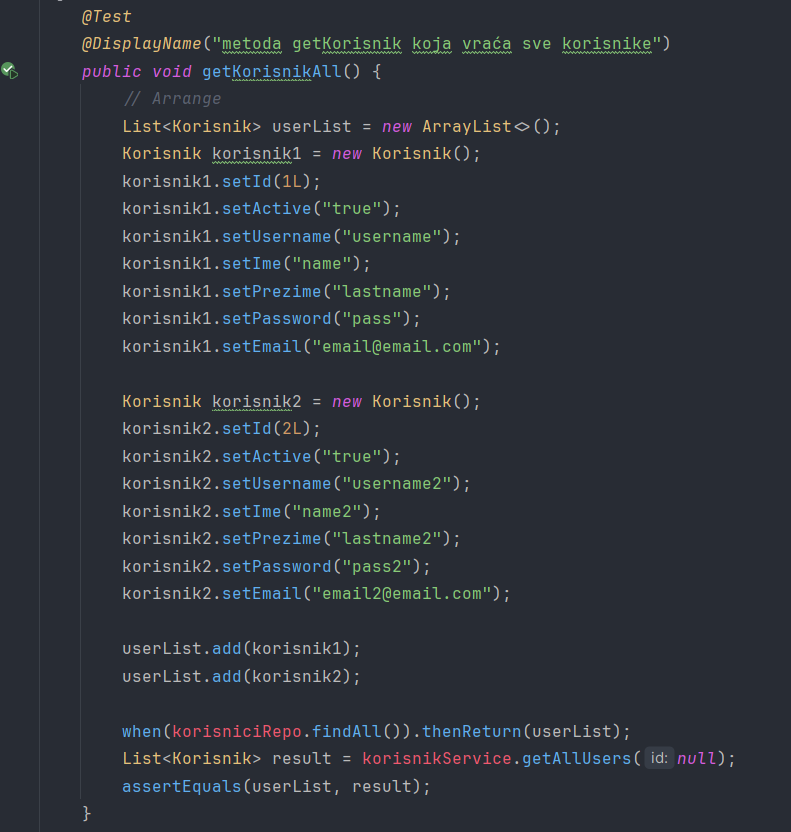
\includegraphics[scale=0.5]{slike/allUsers.PNG} %veličina slike u odnosu na originalnu datoteku i pozicija slike
			\centering
			\caption{Registracija novog korisnika}
			\label{fig:implementacija}
		\end{figure}
		
		\textbf{Test 6: Pregled svih prijava u sustavu}\\
			\\ U predzadnjem provedenom testu kreirane su nove prijave. Cilj je bio iz baze podataka izvući sve porstojeće prijave u sustavu kako bi se provjerila točnost njihovog zapisa u bazi podataka.
			
			\begin{figure}[H]
			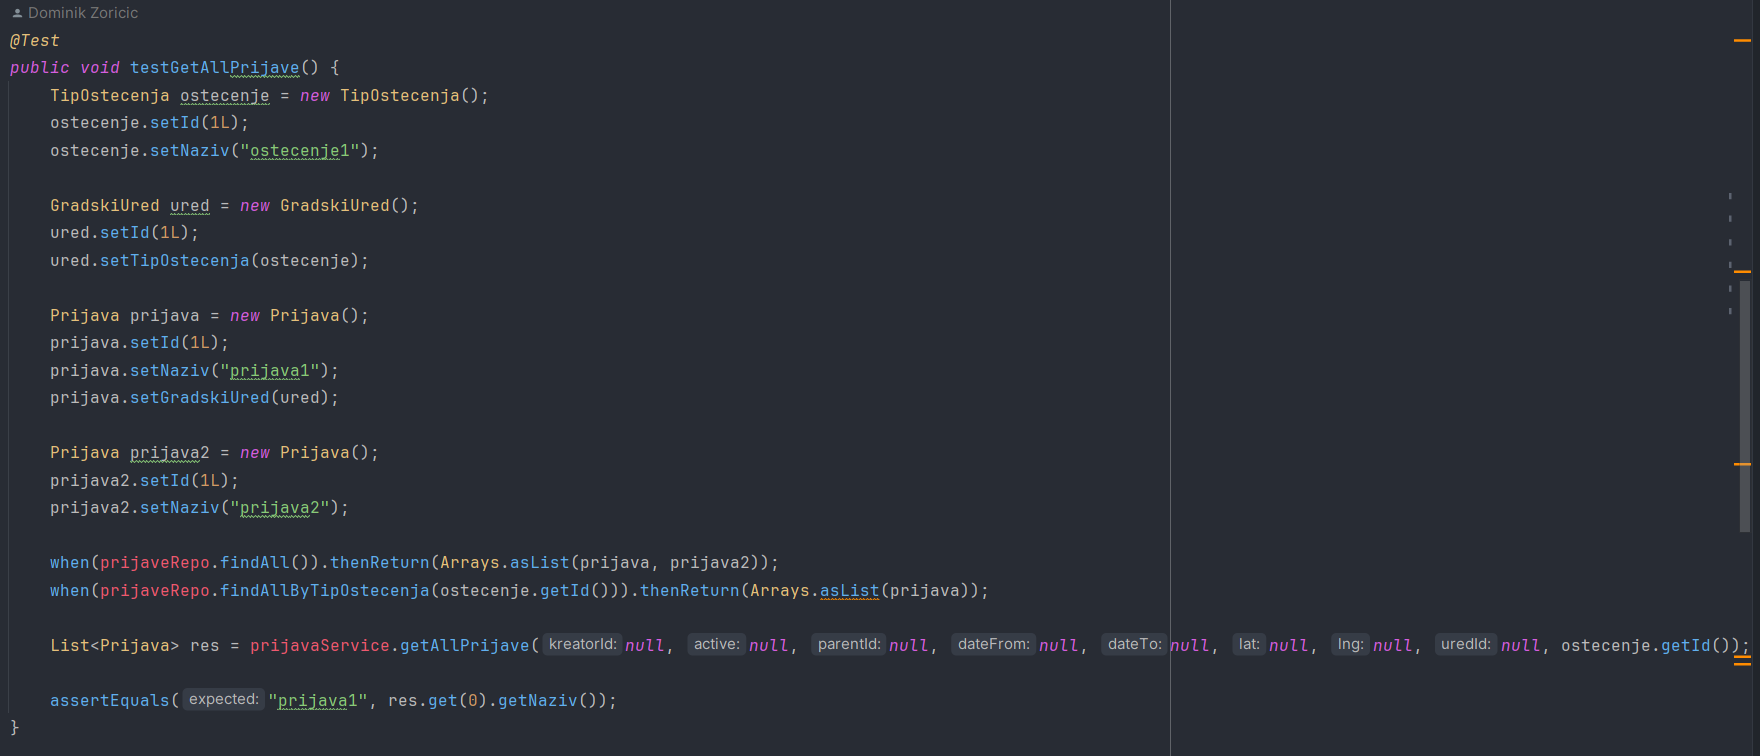
\includegraphics[scale=0.5]{slike/svePrijave.PNG} %veličina slike u odnosu na originalnu datoteku i pozicija slike
			\centering
			\caption{Pretraga svih prijava regsitriranih u bazi podataka}
			\label{fig:implementacija}
		\end{figure}
		
		\textbf{Test 7: Dodavanje nove prijave u sustav}\\
			\\ U zadnjem provedenom testu kreirane su nove prijave. Cilj je bio potvrditi postojanost zapisa nove prijave u bazi podataka.
			
			\begin{figure}[H]
			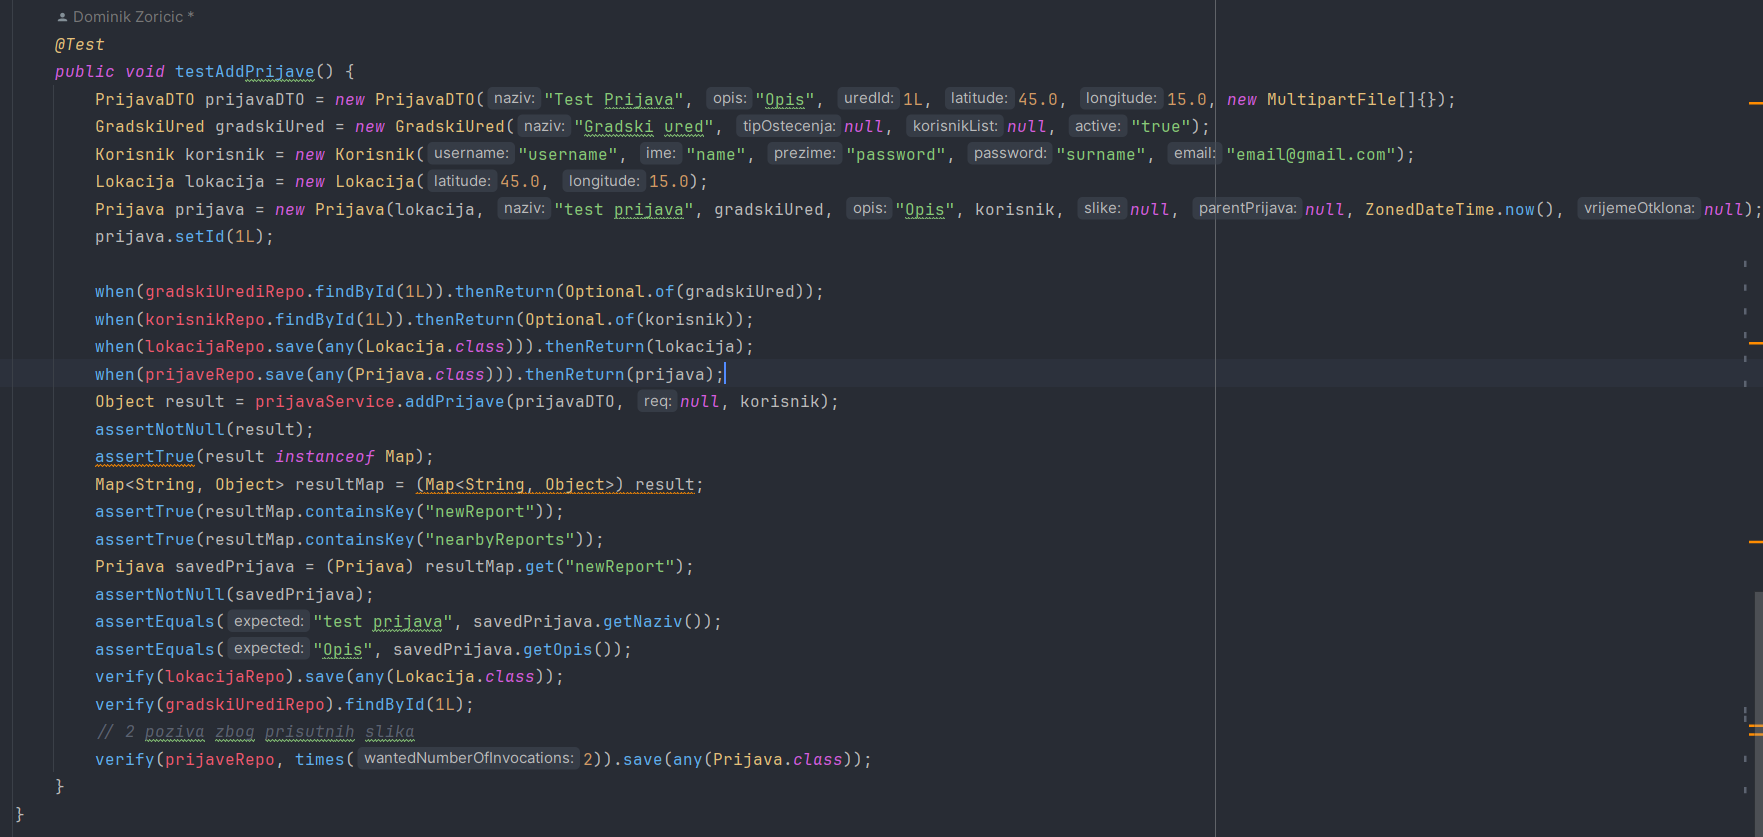
\includegraphics[scale=0.5]{slike/addPrijava.PNG} %veličina slike u odnosu na originalnu datoteku i pozicija slike
			\centering
			\caption{Kreacija novih prijava u sustavu}
			\label{fig:implementacija}
		\end{figure}
			
			
			
			\subsection{Ispitivanje sustava}
			
			 \textit{Potrebno je provesti i opisati ispitivanje sustava koristeći radni okvir Selenium\footnote{\url{https://www.seleniumhq.org/}}. Razraditi \textbf{minimalno 4 ispitna slučaja} u kojima će se ispitati redovni slučajevi, rubni uvjeti te poziv funkcionalnosti koja nije implementirana/izaziva pogrešku kako bi se vidjelo na koji način sustav reagira kada nešto nije u potpunosti ostvareno. Ispitni slučaj se treba sastojati od ulaza (npr. korisničko ime i lozinka), očekivanog izlaza ili rezultata, koraka ispitivanja i dobivenog izlaza ili rezultata.\\ }
			 
			 \textit{Izradu ispitnih slučajeva pomoću radnog okvira Selenium moguće je provesti pomoću jednog od sljedeća dva alata:}
			 \begin{itemize}
			 	\item \textit{dodatak za preglednik \textbf{Selenium IDE} - snimanje korisnikovih akcija radi automatskog ponavljanja ispita	}
			 	\item \textit{\textbf{Selenium WebDriver} - podrška za pisanje ispita u jezicima Java, C\#, PHP koristeći posebno programsko sučelje.}
			 \end{itemize}
		 	\textit{Detalji o korištenju alata Selenium bit će prikazani na posebnom predavanju tijekom semestra.}
			
			\eject 
		
		
		\section{Dijagram razmještaja}
			
			 Dijagram razmještaja opisuje topologiju virtualnih i fizičkih čvorova i komunikacijske puteve između istih. U našem slučaju sustav je temeljen na klijent-poslužitelj odnosu u kojem klijentsko računalo http protokolom razmjenjuje podatke sa serverskim uređajem. Serverska je strana implemenirana pomoću web servisa Render.
			 
			 \begin{figure}[H]
			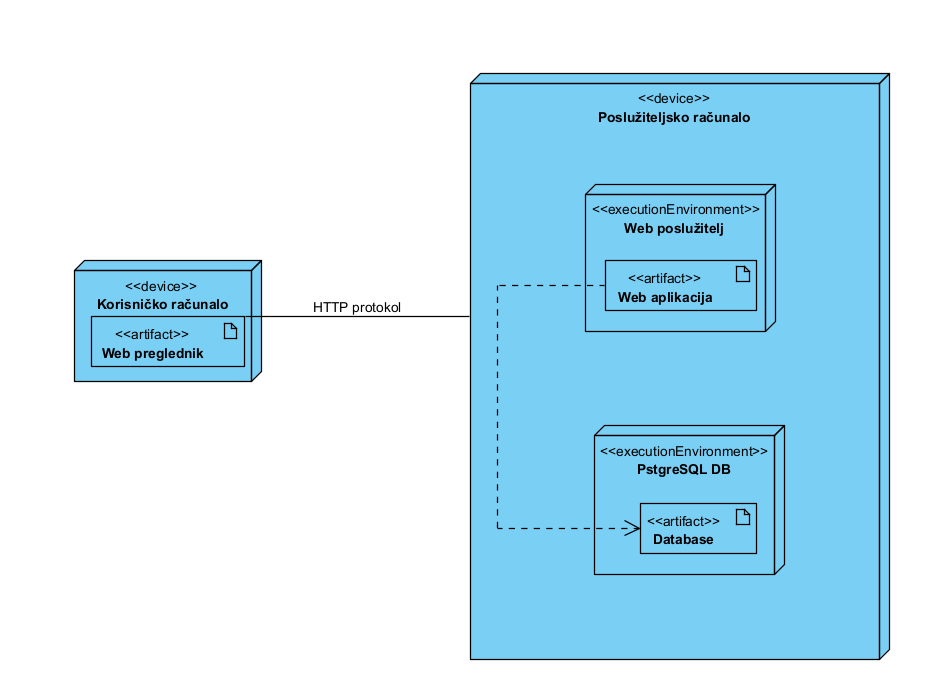
\includegraphics[scale=0.5]{slike/deploymentDiagram.PNG} %veličina slike u odnosu na originalnu datoteku i pozicija slike
			\centering
			\caption{Dijagram razmještaja}
			\label{fig:implementacija}
		\end{figure}
			
			\eject 
		
		\section{Upute za puštanje u pogon}
		
			\subsection{Konfiguracija frontenda}
			Pri konfiguraciji frontenda na poslužitelju Render potrebno je GitHub račun spojiti s Renderom. Idući je korak kreirati novi servis i odabrati projekt Gradska šteta. Regija je Frankfurt (EU Central), za root directory se odabire frontend. Environment se treba postaviti na Node, dok je build command potrebno postaviti na npm run build, a start command na npm run server. Zadnji korak je postaviti evnironment varijable ka na idućoj slici i kliknuti Create Web Server.
			
			
			\begin{figure}[H]
			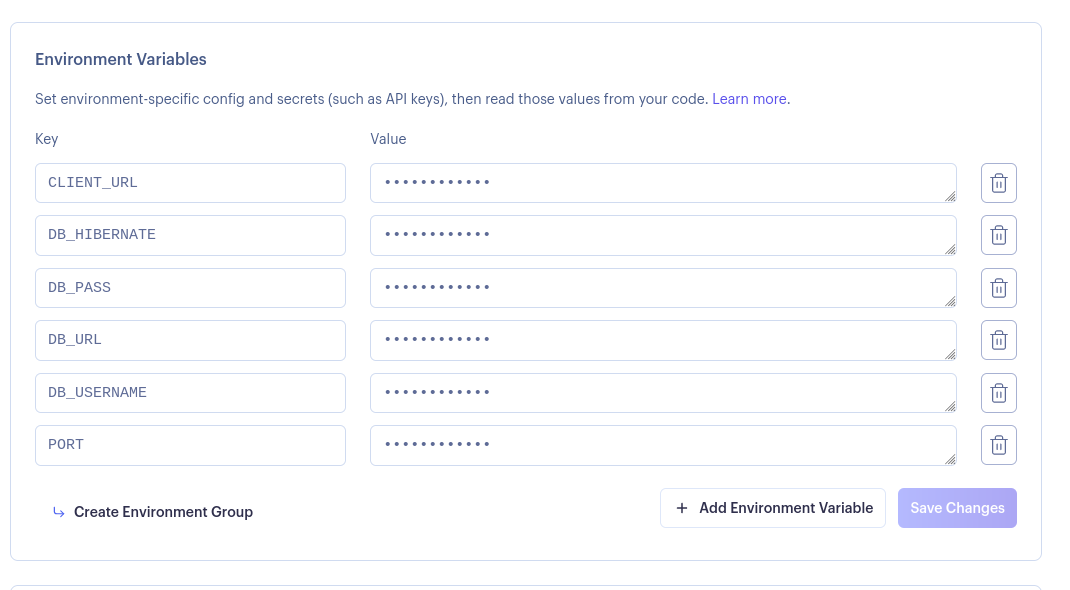
\includegraphics[scale=0.4]{slike/frontendEnvironment.PNG} %veličina slike u odnosu na originalnu datoteku i pozicija slike
			\centering
			\caption{Environment varijable za frontend dio}
			\label{fig:implementacija}
		\end{figure}
		
		\subsection{Konfiguracija backenda}
			
			Pri konfiguraciji backenda na poslužitelju Render potrebno je GitHub račun spojiti s Renderom. Idući je korak kreirati novi servis i odabrati projekt Gradska šteta. Kao regiju treba odabrati Frankfurt (EU Central), za root directory se odabire backend. Dockerfile se nalazi u backend direktoriju (/backend), a Docker Build Context directory je /backend. Na idućoj slici su prikazane environment varijable koje treba postaviti i kliknuti na Create Web Server.
			
			\begin{figure}[H]
			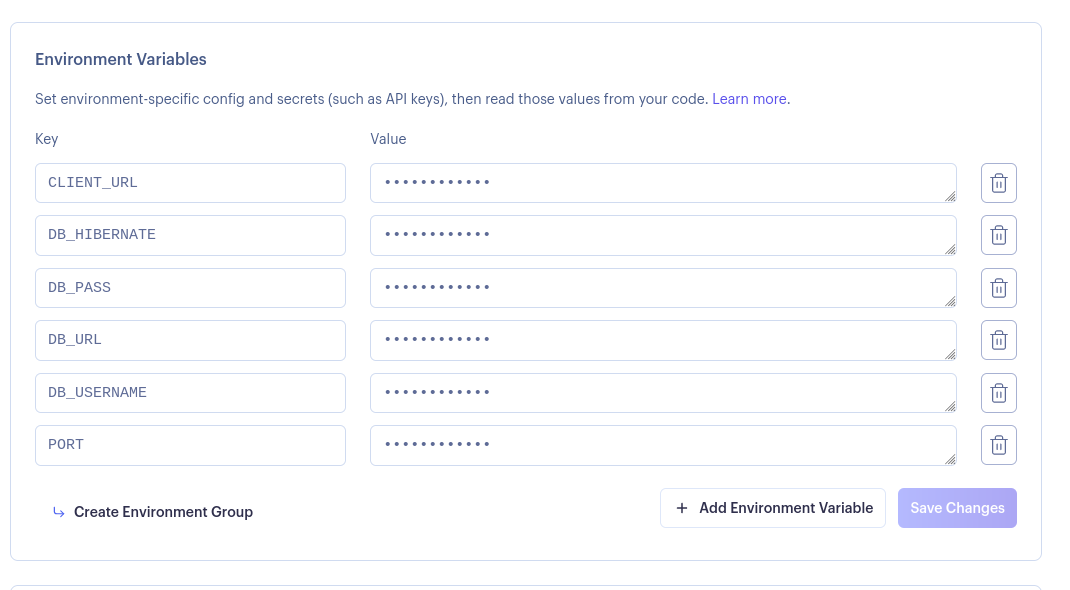
\includegraphics[scale=0.4]{slike/backendEnvironment.PNG} %veličina slike u odnosu na originalnu datoteku i pozicija slike
			\centering
			\caption{Environment varijable za backend dio}
			\label{fig:implementacija}
		\end{figure}
		
		\subsection{Konfiguracija baze podataka}
			
			Pri konfiguraciji poslužitelja baze podataka na Renderu potrebno je postaviti ime baze zajedno sa imenom korisnika baze. Kao regiju postavizi Frankfurt(EU Central) i dovršiti kreiranje sa klikom na Create Database. Environment varijable prikazane su na slici \ref{fig:implementacijaBaze}.
			
			\begin{figure}[H]
			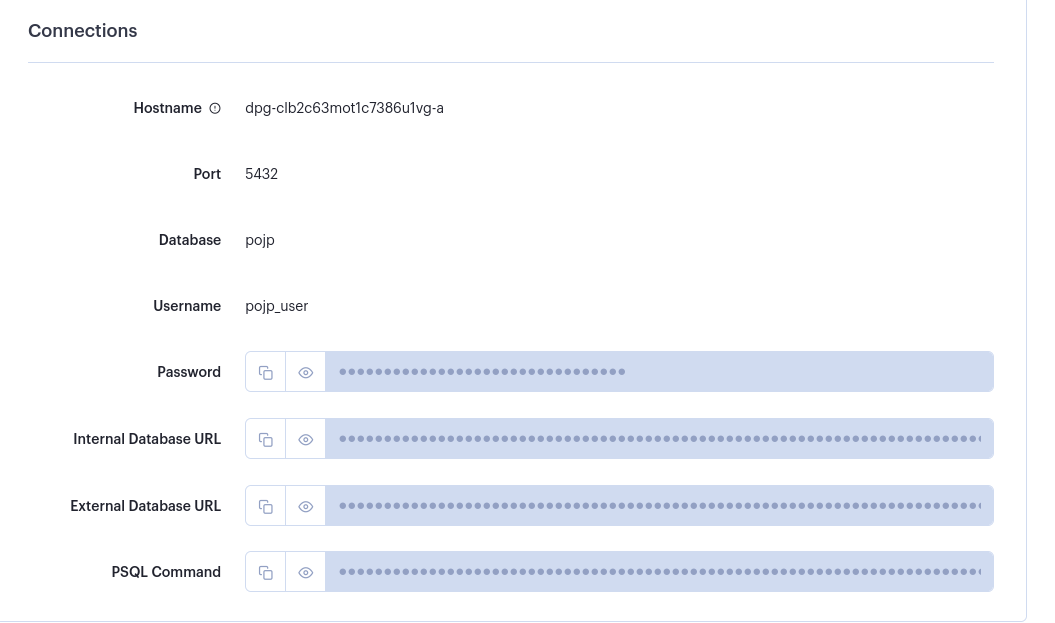
\includegraphics[scale=0.4]{slike/bazaEnvironment.PNG} %veličina slike u odnosu na originalnu datoteku i pozicija slike
			\centering
			\caption{Environment varijable za bazu podataka}
			\label{fig:implementacijaBaze}
		\end{figure}
			
			\eject 